\documentclass{llncs}

\usepackage{mathpartir}
\usepackage{graphicx}
\usepackage{color}
\usepackage[tight]{subfigure}

\newcommand{\goesto}[1][]{\stackrel{#1}{\rightarrow}}
\newcommand{\set}[1]{ \{ #1 \} }
\newcommand{\MATHID}[1]{\ensuremath{\mathit{#1}}}


%%%%%%%%%%%%%%%%%%%% DPHILS EXAMPLE %%%%%%%%%%%%%%%%%
\newcommand{\get}{\MATHID{get}}
\newcommand{\release}{\MATHID{rel}}
\newcommand{\use}{\MATHID{use}}
\newcommand{\free}{\MATHID{free}}

\newcommand{\prio}{\MATHID{\prec}}

\newcolumntype{L}[1]{>{\raggedright\let\newline\\\arraybackslash\hspace{0pt}}m{#1}}
\newcolumntype{C}[1]{>{\centering\let\newline\\\arraybackslash\hspace{0pt}}m{#1}}
\newcolumntype{R}[1]{>{\raggedleft\let\newline\\\arraybackslash\hspace{0pt}}m{#1}}

\newcommand{\rerl}{\texttt{RERL}\xspace}






\makeatletter
\renewcommand\section{\@startsection{section}{1}{\z@}%
                       {-8\p@ \@plus -4\p@ \@minus -4\p@}%
                       {6\p@ \@plus 4\p@ \@minus 4\p@}%
                       {\normalfont\large\bfseries\boldmath
                        \rightskip=\z@ \@plus 8em\pretolerance=10000 }}
\renewcommand\subsection{\@startsection{subsection}{2}{\z@}%
                       {-8\p@ \@plus -4\p@ \@minus -4\p@}%
                       {6\p@ \@plus 4\p@ \@minus 4\p@}%
                       {\normalfont\normalsize\bfseries\boldmath
                        \rightskip=\z@ \@plus 8em\pretolerance=10000 }}
\renewcommand\subsubsection{\@startsection{subsubsection}{3}{\z@}%
                       {-4\p@ \@plus -4\p@ \@minus -4\p@}%
                       {-1.5em \@plus -0.22em \@minus -0.1em}%
                       {\normalfont\normalsize\bfseries\boldmath}}
\makeatother
\setlength{\belowcaptionskip}{-10pt}


\sloppy
\title{Autonomous Learning  of Correctness-At-Runtime in Infinite State Spaces}

\author{Haitham Bou-Ammar, Mohamad Jaber, Mohamad Nassar}


\graphicspath{{./figs/}}
\begin{document}
\maketitle

\begin{abstract}
We introduce a novel framework for runtime enforcement of safe executions in component-based systems with multi-party interactions modeled using BIP. Our technique frames runtime enforcement as a sequential decision making problem and presents two alternatives for learning optimal strategies that ensure fairness between correct traces. We target both finite and infinite state-spaces. In the finite case, we guarantee that the system avoids bad-states by casting the learning process as a one of determining a fixed point solution that converges to the optimal strategy. Though successful, this technique fails to generalize to the infinite case due to need for building a dictionary, which quantifies the performance of each state-interaction pair. As such, we further contribute by generalizing our framework to support the infinite setting. Here, we adapt ideas from function approximators and machine learning to encode each state-interaction pairs' performance. In essence, we autonomously learn to abstract similar performing states in a relevant continuous space through the usage of deep learning. 
We assess our method empirically by presenting a fully implemented tool, so called \rerl. Particularly, we use \rerl to: 1) enforce deadlock freedom on a dining philosophers benchmark, and 2) allow for pair-wise synchronized robots to autonomously achieve consensus within a cooperative multi-agent setting. 
\end{abstract}


\section{Introduction}
Building correct and efficient software systems in a timely manner is still a very challenging task despite the existence of plethora of techniques and methods. For instance, correctness can be ensured using static analysis such as model checking or dynamic analysis such as runtime verification. Static analysis mainly suffers from state-space explosion where as dynamic analysis suffers from its accuracy (reachability cover) and efficiency.  
%
On the other hand, software synthesis, correct-by-design, was introduced to automatically generation implementation from high-level designs. However, correct-by-design was proven to be NP-hard~\cite{PnueliR89} in some cases and undecidability~\cite{PnueliR90} in some main classical automatic synthesis problems. 

Additionally, it is desirable to relax the developer task by giving the option introduce additional behaviors w.r.t. a given specification. Although,  this relaxation would drastically simplifies the development process, it may introduce errors. 

%
In this paper, we introduce a new runtime enforcement technique that takes a software system with additional behaviors and uses machine machine learning and dynamic analysis to synthesis more accurate behaviors, i.e., remove the extra ones w.r.t. input specification. We apply our method to component-based systems with multi-party interactions modeled using BIP. Our technique frames runtime enforcement as a sequential decision making problem and presents two alternatives for learning optimal strategies that ensure fairness between correct traces. That is, the policy should not prioritize correct traces. We target both finite and infinite state-spaces. In the finite case, we guarantee that the system avoids bad-states by casting the learning process as a one of determining a fixed point solution that converges to the optimal strategy. Though successful, this technique fails to generalize to the infinite case due to need for building a dictionary, which quantifies the performance of each state-interaction pair. As such, we further contribute by generalizing our framework to support the infinite setting. Here, we adapt ideas from function approximators and machine learning to encode each state-interaction pairs' performance. In essence, we autonomously learn to abstract similar performing states in a relevant continuous space through the usage of deep learning. 
We assess our method empirically by presenting a fully implemented version in RERL. Particularly, we use RERL to: 1) enforce deadlock freedom on a dining philosophers benchmark, and 2) allow for pair-wise synchronized robots to autonomously achieve a consensus within a cooperative multi-agent setting. 


\section{Related work}
\label{sec:rw}
Runtime enforcement of component-based systems was introduced in~\cite{CharafeddineEFJ15} to ensure the correct runtime behavior (w.r.t. a formal specification) of a system. 
The authors define series of transformations to instrument a component-based system described in the BIP framework. The instrumented system allows to observe and avoid any error in the behavior of the system. 
The proposed method was fully implemented in RE-BIP. 
Although, contrarily to our method, the proposed method is sound (i.e., it always avoids bad states), it mainly suffers from two limitations. First, it only considers a 1-step recovery. That is, if the system enters a correct state from which all the reachable states are bad states, the method fails.  Second, the instrumented system introduces a huge overhead w.r.t. original behavior. This overhead would be drastically increased to support more than 1-step recovery. 

In~\cite{PinisettyPTJFM16,PinisettyT16}, the authors introduced a predictive runtime enforcement framework that allows to build an enforcement monitor with or without a-priori knowledge of the system. 
The enforcement monitor ensures that the system complies with a certain property, by delaying or modifying events. The proposed method is theoretical and cannot be applied to real software systems as delaying or modifying events would require an infinite memory and also is not practical in software systems. 

In~\cite{HuangPSW16}, the authors proposed a game-theoretic method for synthesizing control strategies to maximize the resilience of software systems. The method allows the system to not take transition leading to bad states using game-theoretic method. Consequently,  similar to RE-BIP, the proposed approach only allows a 1-step recovery. In other words, they need to do a back propagation from the bad states to re-label all good states as bad states when all their corresponding traces would lead to bad states, which is not feasible in case of infinite-state system. 


Recent work~\cite{genetic1,genetic2,genetic3} establishes techniques to synthesize code using genetic programming.  In particular, the method randomly generates an initial population of programs based on a given configuration and then they apply mutation functions to optimize a given fitness function (w.r.t. specification). Nonetheless, the method was applied to communication protocols without reporting success rates. Moreover, deep learning is much more expressive than genetic programming, which failed to learn complex structures. Moreover, it is not clear how to automatically derive a fitness function from a given specification. 

\section{Behavior, Interaction and Priority (BIP)}
\label{sec:bip}
We recall the necessary concepts of the BIP framework~\cite{bip2}.
BIP allows to construct systems by superposing three layers of design: Behavior, Interaction, and Priority.
The \emph{behavior} layer consists of a set of atomic components represented by transition systems. 
The \emph{interaction} layer provides the collaboration between components. 
Interactions are described using sets of ports. 
The \emph{priority} layer is used to specify scheduling policies applied to the interaction layer, given by a strict partial order on interactions.

\subsection{Atomic Components}
We define \emph{atomic components} as transition systems with a set of ports labeling individual transitions. These ports are used for communication between different components.

\begin{definition}[Atomic Component]
An  {\em atomic component} $B$ is a labeled transition system represented by a triple $(Q,P,\goesto)$ where $Q$ is a set of {\em states}, $P$ is a set of {\em communication ports}, $\goesto\, \subseteq Q\times P\times Q$ is a set of {\em possible transitions}, each labeled by some port.
\end{definition}

For any pair of states $q,q'\in Q$ and a port $p\in P$, we write $q \goesto[p] q'$, iff $(q,p,q')\in\,\goesto$. When the communication port is irrelevant, we simply write $q \goesto q'$. Similarly, $q \goesto[p]$ means that there exists $q'\in Q$ such that $q \goesto[p] q'$. In this case, we say that $p$ is \emph{enabled} in state $q$.

In practice, atomic components are extended with variables. Each variable may be
bound to a port and modified through interactions involving this port. We also
associate a guard and an update function (i.e., action) to each transition. A guard is a
predicate on variables that must be true to allow the execution of the
transition. An update function is a local computation triggered by the
transition that modifies the variables. 

Figure \ref{fig:philo-fork} shows an atomic component $P$ that corresponds to the behavior of a philosopher in the dining-philosopher problem, where $Q = \{e,h\}$ denotes eating and hungry, $P = \{\release, \get\}$ denotes releasing and getting of forks, and $\goesto = \{e \goesto[\release] h, h \goesto[\get] e\}$.


\subsection{Composition Component}
For a given system built from a set of $n$ atomic components $\{B_i = (Q_i, P_i, \goesto_i)\}_{i=1}^n$, we assume that their respective sets of ports are pairwise disjoint, i.e., for any two $i\not= j$ from $\set{1..n}$, we have $P_i \cap P_j = \emptyset$. We can therefore define the set $P = \bigcup_{i=1}^n P_i$ of all ports in the system. An {\em interaction} is a set $a \subseteq P$ of ports. When we write $a = \{p_i\}_{i\in I}$, we suppose that for $i \in I$, $p_i \in P_i$, where $I \subseteq \set{1..n}$.

Similar to atomic components, BIP extends interactions by associating a guard
and a transfer function to each of them. Both the guard and the function are defined over
the variables that are bound to the ports of the interaction. The guard must be
true to allow the interaction. When the interaction takes place, the
associated transfer function is called and modifies the variables.

\begin{figure}[t]
  \begin{center}
    \mbox{
      \subfigure[Philosopher $P$ and fork $F$ atomic components.]{\label{fig:philo-fork}\scalebox{0.35}{\input{figs/philAndFork.pdf_t}}} \quad
      \subfigure[Dining philosophers composite component with four philosophers.]{\label{fig:diningbip}\scalebox{0.3}{\input{figs/diningbip.pdf_t}}}
      }
    \caption{Dining philosophers.}
    \label{fig:diningSpectrum}
  \end{center}
\end{figure}

\begin{definition}[Composite Component]\label{def.bip.composition}
A {\em composite \linebreak component} (or simply {\em component}) is defined by a composition operator parameterized by a set of interactions $\Gamma \subseteq 2^P$.  $B \stackrel{\mathit{def}}{=} \Gamma(B_1,\dots,B_n)$, is a transition system $(Q,\Gamma, \goesto)$, where $Q=\bigotimes_{i=1}^n Q_i$ and $\goesto$ is the least set of transitions satisfying the rule

\begin{mathpar}
\inferrule
{
    a = \{p_i\}_{i\in I}\in \Gamma\\
    \forall i\in I: q_i \goesto[p_i]_i q'_i\\
    \forall i\not\in I: q_i = q'_i\\
}
{
    (q_1,\dots,q_n) \goesto[a] (q'_1,\dots,q'_n)
}
\end{mathpar}
\end{definition}

The inference rule says that a composite component $B=\Gamma(B_1,\dots,B_n)$ can
execute an interaction $a\in \Gamma$, iff for each port $p_i\in a$, the
corresponding atomic component $B_i$ can execute a transition labeled with
$p_i$; the states of components that do not participate in the interaction stay
unchanged. 

Figure~\ref{fig:diningbip} illustrates a composite component $\Gamma(P_0, P_1, P_2, P_3, F_0, F_1, F_2, F_3)$, where each $P_i$ (resp. $F_i$)  is identical to component $P$ (resp. $F$) in Figure
\ref{fig:philo-fork} and $\Gamma = \Gamma_\get \, \cup \, \Gamma_\release$, where $\Gamma_\get = \bigcup_{i=0}^{3} \{P_i.\get, F_i.\use_l, F_{(i+1) \% 4}.use_r\}$ and $\Gamma_\release = \bigcup_{i=0}^{3}\{P_i.\release, F_i.\free_l, F_{(i+1)\%4}.free_r\}$. 


Notice that several distinct interactions can be enabled at the same time, thus introducing non-determinism in the product behavior. One can add priorities to reduce non-determinism. In this case, one of the interactions with the highest priority is chosen non-deterministically.

\begin{definition}[Priority]
  \label{defn:priority}
  Let $C = (Q,\Gamma,\goesto)$ be the behavior of the composite component $\Gamma(\{B_1, \ldots, B_n\})$.  A {\em priority model} $\prio$ is a
  strict partial order on the set of interactions $\Gamma$. Given a priority model $\prio$, we
  abbreviate $(a,a')\in \prio$ by $a \prec a'$. Adding the priority model $\prio$ over $\Gamma(\{B_1, \ldots, B_n\})$ defines a new composite component $B = \prio\big(\Gamma(\{B_1, \ldots, B_n\})\big)$ noted $\pi(C)$ and whose behavior is defined by $(Q, \Gamma, \goesto_\prio)$, where $\goesto_\prio$ is the least set of transitions satisfying the following rule:
\begin{mathpar}
\inferrule*
	{
      q \goesto[a] q' \and
      \neg\big(\exists a'\in \Gamma,\exists q''\in Q: a \prec a' \wedge q \goesto[a'] q'' \big)
    }
    {
      q \goesto[a]_\prio q'
    }
\end{mathpar}
\end{definition}
%
An interaction $a$ is enabled in $\pi(C)$ whenever $a$ is enabled in $C$ and $a$ is maximal according to $\pi$ among the active interactions in $C$.


BIP provides both centralized and distributed implementations. In the centralized implementation,
a centralized engine guarantees to execute only one interaction at a time, and thus conforms to the operational semantics of the BIP.  The main loop of the BIP engine consists of the following steps:
\begin{enumerate}
\item Each atomic component sends to the engine its current
location.
\item The engine enumerates the list of interactions in the system,
selects the enabled ones based on the current location
of the atomic components and eliminates the ones
with low priority.
\item The engine non-deterministically selects an interaction
out of the enabled interactions.
\item Finally, the engine notifies the corresponding components
and schedules their transitions for execution.
\end{enumerate}

Alternatively, BIP allows the generation of distributed
implementations~\cite{bip-distributed} where non-conflicting interactions
can be simultaneously executed.

\begin{definition}[BIP system]
\label{def:bipsystem}
A BIP system is a tuple $(B, q_0)$, where $q_0$ is the initial state with $q_0 \in \bigotimes_{i=1}^n Q_i$ being the tuple of initial states of atomic components.
\end{definition}


For the rest of the paper, we fix an arbitrary BIP-system $(B, q_0)$, where  $B = \prio\big(\Gamma(\{B_1, \ldots, B_n\})\big)$ with semantics $C = (Q, \Gamma, \goesto)$.

We abstract the execution of a BIP system as a trace.
%
\begin{definition}[BIP trace]
\label{def:trace-global}
A BIP trace $\rho = (q_0 \cdot a_0 \cdot q_1 \cdot a_1 \cdots q_{i-1} \cdot a_{i-1} \cdot q_i)$ is an alternating sequence of states of $Q$ and interactions in $\Gamma$; where $q_k \xrightarrow{a_k} q_{k+1} \in \rightarrow$, for $k \in [0, i-1]$.
\end{definition}

Given a trace $\rho = (q_0 \cdot a_0 \cdot q_1 \cdot a_1 \cdots q_{i-1} \cdot a_{i-1} \cdot q_i)$, 
$\rho^q_i$ (resp. $\rho^a_i$) denotes the $i^\text{th}$ state (resp. interaction) of the trace, i.e., $q_i$ (resp. $a_i$). Also, $\bm{\rho}(C)$ denotes the set of all the traces of an LTS $C$. 


\section{Problem Definition \& Methodology }
We frame the problem of run time enforcement as a sequential decision making (SDM) one, by which the BIP engine has to be guided to select the set of interactions over an extended execution traces that maximize a cumulative return.  We formalize SDMs as the following five-tuple $\left \langle Q, \tilde{Q},\Gamma, \rightarrow, {R}_{+}, {R}_{-}, \gamma \right\rangle$.  Here, $Q$ represents the set of all possible states, $\tilde{Q} \subseteq Q$ the set of ``bad'' states that need to be avoided, $\Gamma$ the set of allowed interactions, and $\rightarrow$ representing the transition model. $R_{+}$ and ${R}_{-}$ are two positive and negative scalar parameter, which allow us to define the reward function quantifying the selection of the engine.
Clearly, the engine gets rewarded when in a state $q \notin \tilde{Q}$, while penalized if $q \in \tilde{Q}$. Using this intuition, one can define a reward function of the states written as: 


\begin{displaymath}
   \mathcal{R}(q) = \left\{
     \begin{array}{lr}
       R_{+} & :  q \notin \tilde{Q} \\
       R_{-} & : q \in \tilde{Q}.
     \end{array}
   \right.
\end{displaymath} 
Given the above reward definition, we finally introduce $\gamma \in [0,1)$ to denote the discount factor specifying the degree to which rewards are discounted over time as the engine interacts with each of the components. 

At each time step $t$, the engine observes a state $q_{t} \in Q$ and must choose an interaction $a_{t} \in \mathcal{A}_{q_t} \subseteq \Gamma$, transitioning it to a new state $q_{t} \goesto[a_{t}]q_{t+1}$ as given by $\rightarrow$ and yielding a reward $\mathcal{R}\left(q_{t+1}\right)$, where $\mathcal{A}_{q_t}$ denotes all enabled interactions from state  $q_{t}$, i.e., $\mathcal{A}_{q_t} = \{a \mid \exists q': q_{t} \goesto[a] q' \in \rightarrow\}$. 
We filter the choice of the allowed interactions, i.e., $\mathcal{A}_{q_t}$, at each time-step by an interaction-selection rule, which we refer to as the policy $\pi$. We extend the sequential decision making literature by defining policies that map between the set of states, $Q$, and any combination of the allowed interactions, i.e., $\pi: Q \rightarrow 2^{\Gamma}$, where for all $q \in Q: \pi(q) \subseteq\mathcal{A}_{q}$.
Consequently, the new behavior of the composite component, guided by the policy $\pi$, is defined by $C_\pi = (Q, \Gamma, \goesto_\pi)$, where $\goesto_\pi$ is the least set of transitions satisfying the following rule:
\begin{mathpar}
\inferrule*
	{
      q \goesto[a] q' \and
      a \in \pi(q)
    }
    {
      q \goesto[a]_\pi q'
    }
\end{mathpar}

The goal now is to find an optimal policy $\pi^{\star}$ that maximizes the \emph{expected} total sum of the rewards it receives in the long run, while starting from an initial state $q_{0} \in Q$. We will evaluate the performance of a policy $\pi$ by:
\begin{equation}
\label{Eq:ValueOne}
\texttt{eval}({\pi}|q_{0}) = \mathbb{E}_{\bm{\rho}(C_\pi)} \left[\sum_{t=0}^{T} \gamma^{t}\mathcal{R}(q_{t},a_{t})\right]= \mathbb{E}_{\bm{\rho}(C_\pi)} \left[\sum_{t=0}^{T} \gamma^{t}\mathcal{R}(q_{t+1})\right],
\end{equation}
where  $\mathbb{E}_{\bm{\rho}(C_\pi)}$ denotes the expectation under all the set of all the allowed (by the policy $\pi$) possible traces, and $T$ is the length of the trace. 


Notice that we index the value of the state by the policy $\pi$ to explicitly reflect the dependency of the value on the policy being followed from a state $q_{t}$. Interestingly, the definition of the evaluator asserts that the value of a state $q_{t}$ is the expected instantaneous reward plus the expected discounted value of the next state. Clearly, we are interested in determining the optimal policy $\pi^{\star}$, which upon its usage yields maximized values for any $q_{t} \in Q$. As such our goal is to determine a policy $\pi$ that solves:
\begin{equation*}
\pi^{\star} \equiv \max_{\pi} \texttt{eval}({\pi}|q_{0}). 
\end{equation*}

%In other words, rather than targeting the determination of $\pi^{\star}$ directly, we will seek the \emph{value} of a state $q \in Q$. %Clearly, one can recover the current iteration policy $\pi$ using:
%$
%\pi(q) = \texttt{argmax}_{a}\{V(q') \mid q \goesto[a] q'\}
%$.


Finally, we quantify the performance of the engine being in a state $q_{t}$ using the so-called value function $V: {Q} \rightarrow \mathbb{R}$. Given such a performance measure, we can deduce the policy, $\pi$ as: 
\begin{equation}
\label{Eq:Policy}
\pi(q) = \arg\max_{a} \{V(q') \mid q \goesto[a] q'\}.
\end{equation}

In what comes next, we define two methods capable of computing such performance measures (consequently policies) in both finite as well as infinite state-space. 

\subsection{Finite State-Space - Value Iteration}
Due to the number of possible policies at each time step, it is a challenge to compute the value for all possible options. Instead, we propose the application of a dynamic programming algorithm known as value iteration, summarized in Algorithm~\ref{Algo:VI} to find the optimal policy efficiently. 
\begin{algorithm}[h!]
\caption{Value Iteration for Run Time Enforcement}
\label{Algo:VI}
\begin{algorithmic}[1]
\STATE \textbf{Input:} Initialization of $V_{0}(q)$ for all $q\in Q$, precision parameter $\epsilon$
\WHILE {$|V_{k+1} - V_{k}| \leq \epsilon$}
	\FOR {\textbf{each} $q \in Q$ }
		\FOR {\textbf{each} $a \in \mathcal{A}$}
			\STATE $V_{k+1}(q) = \max_{a} \left[\mathcal{R}(q, a) + \gamma \sum_{q \goesto[a]q^{\prime}}V_{k}(q^{\prime})\right]$
		\ENDFOR
	\ENDFOR
		\STATE k = k+1
\ENDWHILE
\end{algorithmic}
\end{algorithm}

In essence, Algorithm~\ref{Algo:VI} is iteratively updating the value for all states by choosing these actions that maximize the instantaneous rewards, as well as the future information encoded through $V_{k}(q^{\prime})$. Defining the operator $$\mathcal{T}^{\pi} = \max_{a} \left[\mathcal{R}(q, a) + \gamma \sum_{q \goesto[a]q^{\prime}}V_{k}(q^{\prime})\right],$$ one can easily see that the optimal value function is essentially  fixed-point of $V_{k+1} = \mathcal{T}^{\pi}  V_{k}$. Contrary to state-space-exploration algorithms, our method remedies the need to construct the full labeled transition system as we only require the knowledge of the successor state from a given state and action pair with no regard to its reachability properties. Furthermore, notice that though line~3 in Algorithm~\ref{Algo:VI} requires a loop over all states computational time can be highly reduced by following a sampling-based procedure, where fractions of the state-space are considered. Notice, however, the successfulness of the attained policy comes hand-in-hand with the fraction of the state space sampled. In other words, the higher the fraction, the closer to optimality is the policy and vice versa. 




\subsection{Infinite State-Space - Deep Value Iteration}
The methodology detailed so-far suffers when considering infinite state-spaces as it requires exact representation of performance measures and policies. In general, an exact representation can only be achieved by storing distinct estimates of the return for every state-interaction pair. When states are continuous, such exact representations are no longer possible and performance measures need to be represented approximately. 

Approximation in the continuous setting is not only a problem of representation. Two additional types of approximation are needed. Firstly, sample-based approximation is necessary in any of these frameworks. Secondly, the algorithm must repeatedly solve a difficult minimization problem. To clarify, consider Algorithm~\ref{Algo:VI}, where every iteration necessitates a loop over \emph{every state-interaction pair}. When state space contains an infinite number of elements, it is impossible to loop over all pairs in finite time. Instead, a sample-based update that only considers a finite number of such pairs has to be used. %Given these collected samples, the algorithm has then to update the approximate performance measure; a step that entails 

%The usage of sample-based methods in combination with standard machine learning approximators pose additional problems that need to be carefully analyzed. 
%\textbf{Write about experience replay idea, i.e., forgetting and representation} 
In this section, our goal is to develop an algorithm capable of avoiding the problems above. This ultimately leads us to a method for run-time enforcement operating in continuous state spaces. 
To commence, we introduce a function approximator, encoded through a neural network (particularly its weight matrices which we denote by $\bm{\theta}$), to represent state-values. The goal of this approximator is to \emph{autonomously generalize} over the state-space, such that similarly behaving states cluster together. To achieve the aforementioned goal, one is to fit the parameterization, $\bm{\theta}$, of the neural network to obtain high-expected return.  Unfortunately, the direct application of neural networks in the context of run-time enforcement is challenging since the engine itself has to build, through sampling, a \emph{labeled} data set (with states being inputs and state-values as outputs) to train on. To worsen the problem, at no time instance the engine is given the optimal value of a state $q_{t}$. It rather has to determine these through exploring an infinite state-space. 


\begin{algorithm}[h!]
\caption{Deep-Value Iteration for Run Time Enforcement in Continuous States}
\label{Algo:VI2}
\begin{algorithmic}[1]
\STATE Initialize replay memory $\mathcal{D}$ to capacity $N$, and the neural network weights randomly 
\FOR {$\text{episode} = 1 \ \ \text{to} \ \ M$}
\STATE Set initial state to $q_{0}$
\FOR  {$t=1$ \ \ \text{to} \ \ T}
\STATE With some probability $\epsilon$ select a random interaction $a_{t}$
\STATE With a probability $1 - \epsilon$ select $a_{t} = \max_{a} \left[\mathcal{R}(q_{t}, a) + \gamma V(q_{t+1};\bm{\theta})\right]$
\STATE Execute interaction $a_{t}$ and observe reward, $r_{t}$,and successor state $q_{t+1}$
\STATE Store transition $\left(q_{t}, a_{t}, r_{t}, q_{t+1}\right)$ on replay memory $\mathcal{D}$
\STATE Sample random minibatch of transition $\left(q_{j}, a_{j}, r_{j}, q_{j+1}\right)$ of size $N_{2}$ from $\mathcal{D}$ and create output label by 
\begin{displaymath}
   y_{j} = \left\{
     \begin{array}{lr}
       r_{j} & \text{for terminal $q_{j+1}$}\\
        r_{j} + \gamma \max_{a^{\prime}}\left[\mathcal{R}(q_{j+1}, a^{\prime}) + \gamma V(q_{j+1};\bm{\theta})\right]  & \text{for non-terminal $q_{j+1}$}
     \end{array}
   \right.
\end{displaymath} 
\ENDFOR
\STATE Retrain network $N_{2}$ data points with $y_{j}$ being the labels. 
\ENDFOR
\end{algorithmic}
\end{algorithm}
The details of the above process are described in Algorithm~\ref{Algo:VI2}. On a high-level, the algorithm operates in two loops. The first is episode-based, while the second runs for a horizon $T$. At each episode, the engine's goal is to collect relevant labeled data to improve its approximation (encoded through the neural network) of the performance measure, as summarized in lines 5-10 in the algorithm. First, the engine selects an interaction either randomly with a probability $\epsilon$ (i.e., exploration) or by exploiting the current estimate of the performance measure. Next, the engine executes the interaction and stores both the dynamical transition and its usefulness (i.e., reward) in a replay memory data set, $\mathcal{D}$. To ensure that the engine takes learning memory into account, we sample a set of size $N_{2}$ from $\mathcal{D}$ and label them in line~9  in preparation to retrain the original neural network. The process by which we generate these labels is in essence similar to finite value iterator. The main difference, however, is the usage of sample-based transitions to train a neural network.  






%In other words, starting from randomly initialized weights, $\bm{\theta}$, the engine has to 1) gather relevant traces from the environment, and 2) improve its estimate of $\bm{\theta}$ to maximize its return. Having 









%The goal of such a neural net is to enable continuous states by autonomously generalizing similar...




\section{Experimental results}
\label{sec:bench}
In this section, we present \rerl an implementation of our proposed approach and its evaluation in terms of (1) accuracy of avoiding bad states and, (2) compile and runtime efficiency. 
\subsection{Implementation}
\rerl is an implementation of our method with several modules. The implementation is available at \href{http://staff.aub.edu.lb/~mj54/rerl}{http://staff.aub.edu.lb/\~{}mj54/rerl}. 
\rerl~ is equipped with a command line interface that accepts a set of configuration options. 
It takes the name of the input BIP file, a file containing the bad states (explicitly or symbolically) to be avoided,  and optional flags (e.g., discount factor, number of episodes, horizon length), and it automatically generates a C++ implementation of the input BIP system embedded with a policy to avoid bad states. 
\begin{lstlisting}[language=Bash]
> java -jar RERL.jar [options] input.bip output.cpp badStates.txt
\end{lstlisting}

\subsection{Evaluation}
\paragraph{Dining philosophers.} Figure~\ref{fig:diningbench} shows an example of dining philosophers modeled in BIP that may deadlock. A deadlock will arise when philosopher $P_0$ allocates its right fork $F_0$, then philosopher $P_1$ allocates its right fork $F_1$. That is, a deadlock state is defined as the concatenation when all the philosophers allocate their right forks. We used \rerl to enforce deadlock freedom on this example. We vary the number of philosophers from $2$ to $47$ increasing by $5$. The total number of states is equal to $6^{n}$, where $n$ is the number of philosophers. 
Clearly, value iteration method would explode when the number of philosophers is greater than $12$. 
%
As for the deep value iteration, we ran it with $50$ \texttt{epochs}, $50$ hidden neuron units and $5$ as degree of fairness. The degree of fairness was chosen to be consistent with the good ($+1$) and bad reward ($-1$). Then, we run the system until it executes $10^5$ iterations. The normal implementation always enters the deadlock state whereas when we apply deep value iteration the obtained implementation always avoid the deadlock state.  
%
\begin{figure}[t]
\centering
\subfigure[Philosopher\label{fig:philo}]{\scalebox{0.55}{\input{figs/philo.pdf_t}}}
\subfigure[Fork\label{fig:fork}]{\scalebox{0.55}{\input{figs/fork.pdf_t}}}
\subfigure[Dining philosophers in BIP\label{fig:dining}]{\scalebox{0.7}{\input{figs/diningbip-deadlock.pdf_t}}} 
\caption{Dining philosophers with possible deadlock.}
\label{fig:diningbench}
\end{figure}
%
We also evaluated the runtime overhead induced by the policy, which at every computation step needs to do a forward propagation on the trained neural network to select the best next interactions. Moreover, we compare this overhead against RE-BIP, a tool-set to enforce properties in BIP systems, but which is limited to only a one-step recovery. In this example, one-step recovery is sufficient to avoid deadlock, however, as we will see later it fails in the second benchmark as a $k$ step recovery is needed. Table~\ref{tab:execution-times} summarizes the runtime execution times in case of infinite (while varying number of hidden neuron units), i.e., deep value iteration, finite, i.e., value iteration, and RE-BIP. Clearly, the infinite-based implementation drastically outperforms RE-BIP, when the number of hidden neuron units is less than $100$. Although the finite-based outperforms RE-BIP and guarantees to enforce correct execution, it fails when the size of the system becomes large.  
%
\begin{table}
\centering
\caption{Execution times (in seconds).}
{\small
\begin{tabular}{|C{2cm}||C{0.85cm}|C{0.85cm}|C{0.85cm}|C{0.85cm}|C{0.85cm}||C{1.2cm}||C{1.5cm}||}
\hline
\multirow{2}{*}{\textbf{Nb of}} & \multicolumn{5}{c||}{\textbf{Infinite}} & \multirow{2}{*}{\textbf{Finite}} & \multirow{2}{*}{\textbf{RE-BIP}}  \\ \cline{2-6}
\textbf{Philo.} & 10		& 50		&100 &   500 &    1000  &  &   \\ \hline\hline
\cellcolor{black!10}$2$			& 0.7		& 2.8		&5.5 &    27 &     55  &    1.2&     29  \\ \hline 
\cellcolor{black!10}$7$			&1.4		&6		&11.3 &   58  &    130  &   12.2 &   72  \\ \hline
\cellcolor{black!10}$12$		& 2.3		&9 		&17.5 &   90     & 186     &43  &    122 \\ \hline
\cellcolor{black!10}$17$		& 3			&11.8		&23.2&   121   &   251  &   NA   &   173    \\ \hline
\cellcolor{black!10}$22$		& 3.9		&15.6		&29.3&   154   &   322  &   NA   &   269 \\ \hline
\cellcolor{black!10}$27$		& 5.5		& 18.7		&35 &     190   &  405   &  NA   &   301 \\ \hline
\cellcolor{black!10}$32$		& 5.9		& 22.5		&41.8&    229  &   491   &  NA  &    407 \\ \hline
\cellcolor{black!10}$37$		& 7.1		& 25 		& 48.5&    279  &   567  &   NA  &    450 \\ \hline
\cellcolor{black!10}$42$		& 7.7		& 28.2		&54.9&   325  &   648  &   NA    &  566 \\ \hline
\cellcolor{black!10}$47$		&	 9.7			& 32.6		&60.5&    396   &  764  &   NA   &   652 \\ \hline
\end{tabular}
}
\label{tab:execution-times}
\end{table}
%

\paragraph{Pair-wise synchronized robots.} 
In this benchmark, we model a set of robots placed on a map of size $n \times n$. Initially, all robots are placed at position $(0, 0)$. We consider that robots can only move up or to the right, that is, cannot go back after taking a move.
%
\begin{figure}
%\begin{figure}[h]
\centering
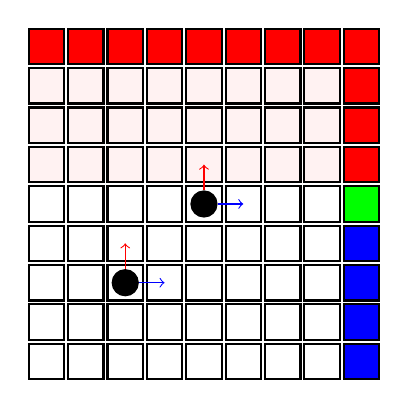
\begin{tikzpicture}
    [%%%%%%%%%%%%%%%%%%%%%%%%%%%%%%
        box/.style={rectangle,draw=black,thick,inner sep=0pt,minimum size=0.45cm},
    ]%%%%%%%%%%%%%%%%%%%%%%%%%%%%%%

\foreach \x in {0,0.5, ..., 4}{
    \foreach \y in {0,0.5, ..., 4}
        \node[box] at (\x,\y){};
}

\foreach \x in {0,0.5, ..., 4}{
        \node[box, fill=red] at (\x,4){};
}

\foreach \y in {2.5,3, ..., 4}{
    \node[box, fill=red] at (4,\y){};
}

\foreach \y in {0,0.5, ..., 1.5}{
    \node[box, fill=blue] at (4,\y){};
} 

\node[box, fill=green] at (4,2){};


\foreach \x in {0,0.5, ..., 3.5}{
    \foreach \y in {2.5,3, ..., 3.5}
        \node[box, fill=red!5] at (\x,\y){};
}
  \node[box] (robot1) at (2,2){};
   \node[box] (robot2) at (1,1){};

  \node[draw, circle, fill=black] (robot11) at (robot1.center) {};
    \node[draw, circle, fill=black] (robot21) at (robot2.center) {};
\draw[->, red] (robot11) -- (2, 2.5);
\draw[->, blue] (robot11) -- (2.5, 2);

\draw[->, red] (robot21) -- (1, 1.5);
\draw[->, blue] (robot21) -- (1.5, 1);
\end{tikzpicture}
\caption{Map of pair-wise synchronizing robots}
\label{fig:map-robots}
\end{figure}
%
Moreover, robot $i$ must synchronize with either robot $i-1$ or $i+1$ (modulo the number of robots) in order to move and both must move with the same direction. Clearly, this would require to create controllers to allow robots to follow that specification. The state of each robot can be modeled by two integers denoting the current position of the robot. We also assume the grid has mines (i.e., bad states) at the top row and the top half most left of the map (i.e., red places in Figure~\ref{fig:map-robots}). 
%
Bottom half most left places are considered safe. Also, we assume that the green location has an exit, which allows the robot to safely exit the map.   

We have modeled robots and their pair-wise synchronization using BIP by allowing them to move to any border locations. Then, we define bad states (i.e., red location) and the goal is to generate a policy that allows robots not go to a bad state. Notice that RE-BIP cannot be used to avoid states as if a robot enters a location on the top half of the map, then 1-step recovery would try all the possible next actions and then fail. For instance, the robot (black circle) on the top has two choices, either moves right or up. The two choices lead the robot to go to a correct state. However, if the robot would take the move up action, it will enter a region where 1-step recovery will fail. 
%
We have tested \rerl using value iteration and deep value iteration by varying the size of the map and the number of robots. Tables~\ref{tab:robots-2},~\ref{tab:robots-4}, \ref{tab:robots-8} depict (1) the success rate when using deep value iteration, value iteration and standard implementation, (2) the time needed to converge in case of deep value iteration, and (3) the number of iterations needed to converge in case of finite value iteration. We ran each configuration $10000$ times to compute the success rate. 
We notice that the value iteration provides a success rate of $100\%$, however, it fails when the size of the system increases. As for the deep value iteration, the system is learning to avoid bad states or states that could lead to bad states and it achieves a high success rate. For instance, if we take a map with $29\times29$ grid size and $8$ robots (i.e., $841^8$ possible states), the standard implementation has $15.1\%$ success rate whereas when using deep value iteration we reach $95.6\%$ success rate. As the state space in this example has a well-defined structure, we only needed $10$ hidden neuron units to train our network by using  deep value iteration algorithm. For this, we notice the efficiency of the compile time, e.g., only $3.6$ seconds are needed to train a system consisting of  $841^8$ states and to reach a $95.6\%$ success rate. 

\begin{table}[t]
\centering
\caption{Evaluation of two robots with different grid sizes.}
{\small
\begin{tabular}{|C{2cm}||C{1.25cm}|C{1.35cm}||C{1.25cm}|C{1.5cm}|C{1.5cm}|}
\hline
\multirow{2}{*}{\textbf{Grid}} & \multicolumn{2}{c||}{\textbf{Infinite}} & \multicolumn{2}{c|}{\textbf{Finite}} & \textbf{Standard}  \\  \cline{2-6}
\textbf{Size} & Succ. \%		& Conv. (s)		&Succ. \% &   Conv. (it.) &    Succ. \%      \\ \hline\hline
\cellcolor{black!10}$5$ & 96.8 & 0.85 &  100 & 7 & 61.7\\ \hline
\cellcolor{black!10}$9$ &	98.6 & 0.98 &	100 & 9& 63.3\\ \hline
\cellcolor{black!10}$13$ &  98.5 & 1.09 &100 & 26& 61.6 \\ \hline
\cellcolor{black!10}$17$ &  99.4 & 1.13 &100 & 34& 58.4\\ \hline
\cellcolor{black!10}$21$ &  99.3 & 1.29 &100 & 42& 63.2\\ \hline
\cellcolor{black!10}$25$ &  99.9 & 1.4 &100 & 50& 59.2\\ \hline
\cellcolor{black!10}$29$  & 99.6 & 1.5 &100 & 58&  61.8\\ \hline
\end{tabular}
}
\label{tab:robots-2}
\end{table}


\begin{table}[t]
\centering
\caption{Evaluation of four robots with different grid sizes.}
{\small
\begin{tabular}{|C{2cm}||C{1.25cm}|C{1.35cm}||C{1.25cm}|C{1.5cm}|C{1.5cm}|}
\hline
\multirow{2}{*}{\textbf{Grid}} & \multicolumn{2}{c||}{\textbf{Infinite}} & \multicolumn{2}{c|}{\textbf{Finite}} & \textbf{Standard}  \\  \cline{2-6}
\textbf{Size} & Succ. \%		& Conv. (s)		&Succ. \% &   Conv. (it.) &    Succ. \%      \\ \hline\hline
\cellcolor{black!10}$5$ & 95.5 & 0.9 &  100 & 7 & 30.5\\ \hline
\cellcolor{black!10}$9$ &	93.9 & 1.08 &	NA & NA& 30.7\\ \hline
\cellcolor{black!10}$13$ &  94.7 & 1.23 &NA & NA& 30.6 \\ \hline
\cellcolor{black!10}$17$ &  97.8 & 1.52 &NA & NA& 28.6\\ \hline
\cellcolor{black!10}$21$ &  97.9 & 1.82 &NA & NA& 29.8\\ \hline
\cellcolor{black!10}$25$ &  98.1 & 2.2 &NA & NA& 30.1\\ \hline
\cellcolor{black!10}$29$  & 97.8 & 2.5 &NA & NA&  30.1\\ \hline
\end{tabular}
}
\label{tab:robots-4}
\end{table}

\begin{table}[t]
\centering
\caption{Evaluation of eight robots with different grid sizes.}
{\small
\begin{tabular}{|C{2cm}||C{1.25cm}|C{1.35cm}||C{1.25cm}|C{1.5cm}|C{1.5cm}|}
\hline
\multirow{2}{*}{\textbf{Grid}} & \multicolumn{2}{c||}{\textbf{Infinite}} & \multicolumn{2}{c|}{\textbf{Finite}} & \textbf{Standard}  \\  \cline{2-6}
\textbf{Size} & Succ. \%		& Conv. (s)		&Succ. \% &   Conv. (it.) &    Succ. \%      \\ \hline\hline
\cellcolor{black!10}$5$ & 92.9 & 1.1 &  NA & NA & 12.2\\ \hline
\cellcolor{black!10}$9$ &	93.9 & 1.5 &	NA & NA& 13.8\\ \hline
\cellcolor{black!10}$13$ &  97.4 & 1.6 &NA & NA& 15.1 \\ \hline
\cellcolor{black!10}$17$ &  95.3 & 2.2 &NA & NA& 13.8\\ \hline
\cellcolor{black!10}$21$ &  94.9 & 3.0 &NA & NA& 17.1\\ \hline
\cellcolor{black!10}$25$ &  94.8 & 3.3 &NA & NA& 14.2\\ \hline
\cellcolor{black!10}$29$  & 95.6 & 3.6 &NA & NA&  15.1\\ \hline
\end{tabular}
}
\label{tab:robots-8}
\end{table}


\section{Conclusions and perspectives}
\label{sec:conclusion}
In this paper, we introduced a new technique that combines static analysis and dynamic analysis with the help of machine learning techniques, in order to ensure the correct execution of software systems. 
Experimental results show that it is possible to learn reachability of bad behaviors by only exploring part of the system. 
For future work, we consider several directions. 
First, we plan to study more expressive properties (e.g., liveness). Second, we consider to generate a partial state semantics, and hence, allow to automatically generate multi-threaded implementations. Third, we consider to generate decentralized policies to facilitate the generation of efficient distributed implementations. 

\bibliographystyle{splncs}
\bibliography{biblio}
\end{document}
